
\documentclass[ucs]{beamer}

\usetheme{GSyC}
%\usebackgroundtemplate{\includegraphics[width=\paperwidth]{gsyc-bg.png}}


\usepackage[greek,spanish]{babel}   %greek permite usar euro 
\usepackage[utf8x]{inputenc}
\usepackage{graphicx}
\usepackage{amssymb} % Simbolos matematicos


% Metadatos del PDF, por defecto en blanco, pdftitle no parece funcionar
   \hypersetup{%
     pdftitle={Administración de Servicios y Aplicaciones},%
     %pdfsubject={Diseño y Administración de Sistemas y Redes},%
     pdfauthor={GSyC},%
     pdfkeywords={},%
   }
%


% Para colocar un logo en la esquina inferior de todas las transpas
%   \pgfdeclareimage[height=0.5cm]{gsyc-logo}{gsyc}
%   \logo{\pgfuseimage{gsyc-logo}}


% Para colocar antes de cada sección una página de recuerdo de índice
%\AtBeginSection[]{
%  \begin{frame}<beamer>{Contenidos}
%    \tableofcontents[currentframetitle]
%  \end{frame}
%}



\begin{document}

% Entre corchetes como argumento opcional un título o autor abreviado
% para los pies de transpa
\title[Git]{Git}
%\subtitle{Diseño y Administración de Sistemas y Redes}
\author[GSyC]{Escuela Tec. Sup. Ingeniería Telecomunicación}
\institute{gsyc-profes (arroba) gsyc.es}
\date[2015]{Noviembre de 2015}


%% TÍTULO
\begin{frame}
  \titlepage
  % Oportunidad para poner otro logo si se usó la opción nologo
  % \includegraphics[width=2cm]{logoesp}  
\end{frame}



%% LICENCIA DE REDISTRIBUCIÓN DE LAS TRANSPAS
%% Nota: la opción b al frame le dice que justifique el texto
%% abajo (por defecto c: centrado)
\begin{frame}[b]
\begin{flushright}
{\tiny
\copyright \insertshortdate~\insertshortauthor \\
  Algunos derechos reservados. \\
  Este trabajo se distribuye bajo la licencia \\
  Creative Commons Attribution Share-Alike 4.0\\
}
\end{flushright}  
\end{frame}



%% ÍNDICE
%\begin{frame}
%  \frametitle{Contenidos}
%  \tableofcontents
%\end{frame}


%%---------------------------------------------------------------
\section{Introducción}
%%---------------------------------------------------------------

%%---------------------------------------------------------------
\begin{frame}[fragile]
\frametitle{Introducción a los sistemas de control de versiones}
\begin{itemize}
\item
En cualquier proyecto software de mediano tamaño trabajan muchas personas, en
un número muy grande de
ficheros, fuertemente dependientes entre sí
\item
Los ficheros cambian continuamente, cada fichero irá teniendo distintas
\emph{revisiones}: r23, r24, r25...
\item
Si solo se cuenta con un directorio compartido, los problemas son enormes

Ejemplo 1:
\begin{itemize}
\item
Juan modifica \verb|client.c r24|  y genera \verb|client.c r25|, que interactúa
con \verb|server.c r51|
\item
Pero María edita \verb|server.c r51| que pasa a ser \verb|server.c r52|, introduciendo cambios
que provocan que el cliente deje de funcionar
\end{itemize}
\end{itemize}

\end{frame}


%%---------------------------------------------------------------
\begin{frame}[fragile]
\frametitle{}
Ejemplo 2:
\begin{itemize}
\item
Despues de cientos de revisiones de cada fichero, liberamos (publicamos) la primera versión
del sistema disponible para nuestros usuarios,
\verb|miproducto v1.0|
\item
Liberamos una nueva versión \verb|v1.1|, que incluye funcionalidad adicional, no 
muy bien probada
\item
Aparece un problema en \verb|miproducto v1.0|, por lo que preparamos un parche y liberamos la versión \verb|v1.0.1|
\item
Es necesario aplicar un parche similar a \verb|v1.1|, y con cambios adicionales, liberamos \verb|v1.2|, que ya consideramos
estable
\item
Vamos trabajando en una futura versión \verb|v2.0|, que supondrá un rediseño completo. Pero simultánemente, seguiremos desarrollando
la versión \verb|1.3|
\end{itemize}

%Con todo ello resulta un número de ficheros muy elevado, muy difícil de manejar \emph{a mano}
\end{frame}



%%---------------------------------------------------------------
\begin{frame}[fragile]
\frametitle{}
Resulta evidente la necesidad de un \emph{sistema de control de versiones}, también llamado \emph{repositorio} que permita:
\begin{itemize}
\item
Que cada desarrollador tenga su propia copia local \emph{congelada} del sistema, pero que luego pueda llevar
sus cambios al sistema global (hacer un \emph{commit})
\item
Conocer todos y cada uno de los cambios realizados: autor, fecha, diferencias con el estado anterior, etc
\item
Almacenar todas las revisiones y versiones, para poder recuperar o deshacer cualquiera de ellas
\item
etc etc
\end{itemize}
%git es un sistema distribuido de control de versiones, \emph{aka} sistema de control de código fuente
El uso más habitual es el desarrollo de software, pero es útil para cualquier entorno
donde deseemos controlar los sucesivos estados un sistema de ficheros: ficheros de configuración, documentación
diversa
o incluso nuestro \emph{home}

\end{frame}

%%---------------------------------------------------------------
\begin{frame}[fragile]
\frametitle{Evolución de los sistemas de control de versiones}

VCS: \emph{Version Control System}, aka RCS, \emph{Revision Control System}
\begin{itemize}
\item
Primera generación. RCS (Año 1982). No era un verdadero control de versiones sino
de \emph{revisiones}. El sistema podía gestionar todas las revisiones 
de \verb|server.c|
y 
de \verb|client.c|,
pero no sabía qué revisión de \verb|client.c| era contemporánea a cada revisión de \verb|server.c|
\item
Segunda generación. CVS (Año 1990). Resuelve el problema anterior, entre otros


\end{itemize}


\end{frame}
%%----------------------------------------------
\begin{frame}[fragile]

\begin{itemize}

\item
Tercera generación. SVN (Año 2000). Diversas mejoras: atomicidad, mantenimiento del historial
tras los cambios (renombrar, copiar, mover), mayor eficiencia con los binarios, creación
de ramas, soporte unicode...
\item
Cuarta generación. Sistemas distribuidos de control de versiones 
(DVCS, \emph{Distributed Version Control System}). Git (Linux Torvalds, año 2005). Mercurial (Año 2005).
En principio Git era más potente y Mercurial más sencillo de manejar, pero ambos han
mejorado mucho y actualmente resultan similares
% Otro es bazaar (2005). Lo llevaba canonical. Lo usa emacs. En 2012, 2013 lo han ido abandonando.
\end{itemize}

\end{frame}


%%---------------------------------------------------------------
\begin{frame}[fragile]
\frametitle{Ventajas de git frente a sistemas de generaciones anteriores}
\begin{itemize}
\item
Por ser distribuido, toda la gestión se hace en el repositorio local. Luego, se puede integrar
mediante \emph{push} y \emph{pull} con uno o varios repositorios remotos
\item
Un repositorio es un único directorio, autocontenido, con todo el historial completo.

Eso lo hace muy robusto frente a fallos: aunque es habitual emplear una topología en
estrella con un maestro y varios esclavos, cualquiera de los
esclavos puede reemplazar al maestro
\item
Cada estado se almacena completo. No como la diferencia desde el estado anterior
\end{itemize}

\end{frame}


%%---------------------------------------------------------------
\begin{frame}[fragile]
\frametitle{Otras características de git}
\begin{itemize}
\item
Los commit del repositorio local se pueden modificar y rehacer por completo,
de manera que los commit que subimos al repositorio maestro estén muy cuidados

Pero incluso se pueden subir cosas que modifiquen lo ya subido. O puede
desaparecer parte del historial, creando \emph{commit fantasma}

Los defensores de mercurial critican esta capacidad de \emph{modificar el pasado}
\end{itemize}

\end{frame}


%%---------------------------------------------------------------
\section{Instalación y configuración}
%%---------------------------------------------------------------
%%---------------------------------------------------------------
\begin{frame}[fragile]
\frametitle{Instalación de git}
Para debian y derivados:
\begin{enumerate}
\item
\verb|apt-get update  # Refresca la lista de paquetes|
\item
\verb|apt-get upgrade # Actualiza el sistema|
\item
\verb|apt-get install git-core|
\end{enumerate}

La instalación es el paso 3, los pasos 1 y 2 normalmente son recomendables antes
de instalar cualquier paquete

Naturalmente, esto solo lo puede hacer el administrador. Y en el laboratorio
no será necesario, git ya está instalado

Clientes gráficos:

\begin{itemize}
\item
Aquí veremos como se usa git desde la shell, pero también
podemos instalar clientes gráficos

En Windows y MacOS podemos emplear p.e. \verb|sourcetree|
(\emph{freeware})
\end{itemize}


\end{frame}

%%---------------------------------------------------------------
\begin{frame}[fragile]
\frametitle{Configuración inicial }
\begin{itemize}
\item
Antes de empezar a usar git, es necesario indicar nuestro nombre y correo
electrónico, para que conste en cada commit
\item
Es conveniente añadir algunos \emph{alias}, para simplificar el
uso de las órdenes más habituales
\item
Para todo ello, recomendamos crear un fichero \verb|~/.gitconfig| con el
siguiente contenido, modificando los datos personales:
  \begin{tiny}
  \begin{verbatim}
[alias]
    log2 = log --pretty=format:\"%h %ad | %s%d [%an]\" --graph --date=short
    log3 = log  --pretty=format:\"%h %ad | %s%d [%an]\"  --name-status  --date=short
    log4= log --color --pretty=format:'%Cred%h%Creset -%C(yellow)%d%Creset %s \ 
          %Cgreen(%cr)  %C(bold blue)<%an>%Creset' --abbrev-commit
    ca = commit --all
    caa = commit  --all --amend
    co = checkout 
    br = branch
[user]
    name = Juan García García
    email = juan.garcia@micorreo.com
[push]
    default = matching

  \end{verbatim}
Puedes descargar este fichero
de configuración en
\verb|http://tinyurl.com/nancr6j|

  \end{tiny}
\end{itemize}

\end{frame}



%%---------------------------------------------------------------
\begin{frame}[fragile]
\frametitle{}
\begin{itemize}


\item
Observa que aquí usaremos órdenes como

\verb|git co|,
\verb|git ca|,
\verb|git br|,
\verb|git log2|,

que no son estándar, sino alias personalizados que no funcionarán
a menos que los definas en este fichero

\end{itemize}

\end{frame}


%%---------------------------------------------------------------
\begin{frame}[fragile]
\frametitle{Creación de un repositorio }

Un repositorio es un directorio: normalmente el VCS controla
todos los ficheros (y directorios) de su interior, excepto 
aquellos que no incluyamos


Primero trabajaremos con un repositorio local, 
posteriormente lo integraremos con repositorios remotos

Hay varias formas de crear un repositorio, veremos dos


\begin{itemize}
\item
Creación partiendo de cero
\item
Creación mediante clonación por ssh

Consiste en crear un repositorio en la máquina local que es un clon
de un repositorio que está en una máquina remota a la que tenemos
acceso por ssh
\end{itemize}

Otras posibilidades son la clonación de un directorio local
o la clonación de un directorio remoto a través de http


\end{frame}
%%----------------------------------------------
\begin{frame}[fragile]

\frametitle{Creación partiendo de cero}


Creamos un directorio vacío, entramos dentro e invocamos a \verb|init|
  \begin{footnotesize}
  \begin{verbatim}
mkdir repo01
cd repo01
git init
  \end{verbatim}
  \end{footnotesize}


\end{frame}

\begin{frame}[fragile]
\frametitle{Creación mediante clonación por ssh}
Creamos un directorio vacío y desde el directorio padre
del directorio recién creado, invocamos a \verb|git clone|, pasando como primer argumento la dirección
del repositorio preexistente y como segundo argumento, el directorio (vacío) que acabamos de crear

%git clone ssh://usuario@maquina/var/tmp/repo.padre.git  repo01
  \begin{footnotesize}
  \begin{verbatim}
mkdir repo01
git clone usuario@maquina:/var/tmp/padre.git  repo01
  \end{verbatim}
  \end{footnotesize}


\end{frame}


%%---------------------------------------------------------------
\begin{frame}[fragile]
\frametitle{Ficheros de configuración}
\begin{itemize}
\item
Todo repositorio git tiene un subdirectorio oculto \verb|.git|
que contiene su historial completo. Si copiamos/movemos
el directorio del repositorio junto con el subdirectorio
\verb|.git|, estamos copiando/moviendo el repositorio
completo, con todas sus características
\item
El fichero \verb|.git/config| contiene la configuración de
ese repositorio

Por tanto, git maneja dos ficheros de configuración

\begin{enumerate}
\item
\verb|~/.gitconfig|

Fichero de configuración global, aplicable a todos los repositorios del 
usuario en esa máquina
\item
\verb|.git/config|

Fichero de configuración particular de cada repositorio

p.e. \verb|~/repo01/.git/config|
\end{enumerate}
\end{itemize}

\end{frame}


%%---------------------------------------------------------------
\begin{frame}[fragile]
\frametitle{}
\begin{itemize}
\item
Podemos incluir dentro del repositorio un fichero \verb|.gitignore|, que especifica
qué ficheros se deben ignorar

p.e.

  \begin{footnotesize}
  \begin{verbatim}
*.log
*.out
*.txt~
.*
  \end{verbatim}
  \end{footnotesize}
\end{itemize}

\end{frame}


%%---------------------------------------------------------------
\section{Uso básico del repositorio local}
%%---------------------------------------------------------------

\begin{frame}[fragile]
\frametitle{Estados de un fichero en git}
\begin{minipage}{7cm}
\begin{figure}
\begin{center}
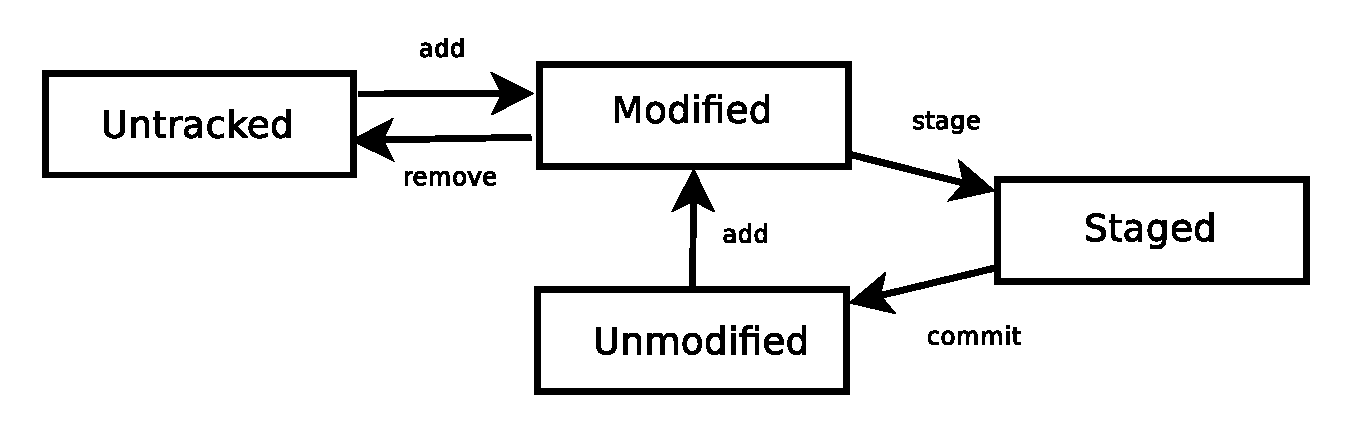
\includegraphics[width=10cm]{figs/estados_git}
\end{center}
\end{figure}
\begin{tiny}
\begin{flushright}
\end{flushright}
\end{tiny}

\end{minipage} \hfill
\

\begin{itemize}
\begin{small}
\item
\emph{untracked}: fichero que el repositorio ignora
\item
\emph{unmodified}: fichero que está en el repositorio
\item
\emph{modified}: fichero del repositorio que ha cambiado, aunque el cambio de momento se ignora
\item
\emph{staged}: fichero del repositorio que ha cambiado, y que será actualizado en el repositorio
en el próximo \emph{commit}
\end{small}
\end{itemize}
\end{frame}


%%---------------------------------------------------------------
\begin{frame}[fragile]
\frametitle{Marcar ficheros para su seguimiento}
Un fichero recién creado o copiado en el directorio, inicialmente
es ignorado por git, su estado es \emph{untracked}

El primer paso será marcarlo para que git lo siga, lo ponemos
en estado "modified"

  \begin{footnotesize}
  \begin{verbatim}
echo "primera linea" > a.txt  
git add a.txt  # Pasa el fichero a "modified"
  \end{verbatim}
  \end{footnotesize}

\end{frame}


%%---------------------------------------------------------------
\begin{frame}[fragile]
\frametitle{Inclusión de ficheros en el repositorio}
Git introduce el estado \emph{modified}, que no tiene 
equivalente en VCS anteriores

Supongamos que trabajo en los ficheros 
\verb|a.py|,
\verb|b.py|,
y
\verb|c.py|

\begin{enumerate}
\item
\verb|a.py|
y
\verb|b.py|
están listos para el commit.
\item
\verb|c.py| todavía no
\item
Quiero hacer ya un commit, sin esperar a terminar \verb|c.py|

\end{enumerate}

¿Cuál es el estado de \verb|c.py|?

\begin{itemize}
\item
No puede ser \emph{unmodified}, porque ya no está como estaba en el commit anterior
\item
No puede ser \emph{staged} porque no quiero incluirlo en el próximo commit
\item
Tampoco quiero pasarlo a \emph{untracked}, porque eso haría que el repositorio
dejase de seguir el fichero (incluyendo la versión que ya está en el repositorio)
\end{itemize}
El estado de 
\verb|c.py|
es \emph{modified}

\end{frame}



%%---------------------------------------------------------------
\begin{frame}[fragile]
\frametitle{}
\begin{itemize}
\item
Como hemos visto, el estado \emph{modified} puede ser conveniente en ciertos escenarios

\begin{enumerate}
\item
Los ficheros modificados automáticamente pasan a
\emph{modified}
\item
Los que queramos llevar al commit, los pasamos a \emph{staged} con la orden \verb|git add|
\item
Hacemos commit
\end{enumerate}


  \begin{footnotesize}
  \begin{verbatim}
git add a.py b.py  # Lleva los ficheros a "staged"
git commit         # Lleva los ficheros a "unmodified"
  \end{verbatim}
  \end{footnotesize}

Para deshacer esto y que un fichero vuelva a 
\emph{modified}

  \begin{footnotesize}
  \begin{verbatim}
git rm --cached b.py
  \end{verbatim}
  \end{footnotesize}

\item
Pero también se puede \emph{vivir sin el estado modified}, como hacían todos los VCS anteriores

  \begin{footnotesize}
  \begin{verbatim}
git commit --all   # Lleva todos los ficheros a "unmodified"
                   # (excepto los "untracked")
  \end{verbatim}
  \end{footnotesize}
O con el alias que hemos definido en \verb|~/gitconfig|
  \begin{footnotesize}
  \begin{verbatim}
git ca
  \end{verbatim}
  \end{footnotesize}

Esto hace commit de todos los ficheros modificados, ignorando la diferencia entre
\emph{modified} y \emph{staged}. 

\end{itemize}

\end{frame}

%%---------------------------------------------------------------
\begin{frame}[fragile]
\begin{itemize}
\item

Por simplificar, en esta asignatura trabajaremos siempre de la segunda forma,

\verb|git ca|

ignorando la diferencia entre \emph{modified} y \emph{staged}

\item
Esto resulta más cómodo porque 
no es necesario hacer un 

\verb|git add| 

para cada fichero en cada commit

Basta con hacer \verb|git add| una sola vez al crear el fichero, para sacarlo del
estado \emph{untracked}
\end{itemize}

\end{frame}



%%---------------------------------------------------------------
\begin{frame}[fragile]
\frametitle{}
Es impresincible que todo commit tenga un comentario

Se puede indicar de dos maneras
\begin{itemize}
\item
Con la opción \verb|-m|

\verb|git ca -m "Modifica tal y cual cosa"|
\item
Sin indicarlo desde la shell

\verb|git ca |

En este caso,  git abrirá nuestro editor por omisión para
que introduzcamos el comentario


\begin{itemize}
\item
El editor por omisión podemos especificarlo definiendo la
variebla de entorno \verb|EDITOR| en el fichero
\verb|~/.bashrc|

  \begin{footnotesize}
  \begin{verbatim}
export EDITOR=vim
  \end{verbatim}
  \end{footnotesize}
\end{itemize}


\end{itemize}

La recomendación es escribir los comentarios en presente y en tercera persona,
como si todos empezaran por \emph{Este commit...}
\end{frame}

%%---------------------------------------------------------------
\begin{frame}[fragile]
\frametitle{Ejemplo }

  \begin{footnotesize}
  \begin{verbatim}
mkdir mi_repo
cd mi_repo
git init  # Creamos el repositorio partiendo de cero
echo "Primera linea" > a.txt
git add a.txt    # Pasa el fichero a "modified"
git ca -m "Crea el primer commit de prueba"
echo "Segunda linea" >> a.txt
git ca -m "Crea el segundo commit de prueba"
  \end{verbatim}
  \end{footnotesize}

%rm -rf mi_repo;mkdir mi_repo; cd mi_repo; git init; echo "Primera linea" > a.txt ; git add a.txt ; git ca -m "Crea el primer commit de prueba";
%echo "Segunda linea" >> a.txt ; git ca -m "Crea el segundo commit de prueba"  ;



Con esto hemos creado un repositorio, le hemos añadido un fichero, hemos hecho un commit, lo 
hemos modificado y hemos realizado un segundo commit
\end{frame}


%%---------------------------------------------------------------
\begin{frame}[fragile]
\frametitle{}
La orden 

\verb|git status|

devuelve el estado de todos los ficheros del directorio actual
y sus subdirectorios

  \begin{scriptsize}
  \begin{verbatim}
koji@mazinger:/tmp/mi_repo$ git status
# En la rama master
nothing to commit, working directory clean
koji@mazinger:/tmp/mi_repo$ echo blabla > b.txt
koji@mazinger:/tmp/mi_repo$ echo "segunda linea" >> a.txt 
koji@mazinger:/tmp/mi_repo$ git status
# En la rama master
# Cambios no preparados para el commit:
#   (use «git add <archivo>...» para actualizar lo que se ejecutará)
#   (use «git checkout -- <archivo>...« para descartar cambios en le directorio de trabajo)
#
#	modificado:   a.txt
#
# Archivos sin seguimiento:
#   (use «git add <archivo>...» para incluir lo que se ha de ejecutar)
#
#	b.txt
no hay cambios agregados al commit (use «git add» o «git commit -a»)

  \end{verbatim}
  \end{scriptsize}

\end{frame}


%%---------------------------------------------------------------
\begin{frame}[fragile]
\frametitle{}
La orden 

\verb|git log|

devuelve el registro de todos los commit del repositorio

  \begin{footnotesize}
  \begin{verbatim}
koji@mazinger:/tmp/mi_repo$ git log
commit 6d6de6bb15bffae7bdd222b661905b14d342db4e
Author: Juan Pérez <jperez@urjc.es>
Date:   Mon Oct 28 18:07:15 2013 +0100

    Crea el segundo commit de prueba

commit 1681c2a4867c759eb1300d2b6514b7996071ab4c
Author: Juan Pérez <jperez@urjc.es>
Date:   Mon Oct 28 18:07:14 2013 +0100

    Crea el primer commit de prueba

  \end{verbatim}
  \end{footnotesize}

\end{frame}



%%---------------------------------------------------------------
\begin{frame}[fragile]
\frametitle{}
En el fichero \verb|~/.gitconfig| hemos creado los alias
\verb|log2, log3| y \verb|log4|, que presentan
diversas variantes de 
\emph{logs} más compactos

  \begin{scriptsize}
  \begin{verbatim}
koji@mazinger:/tmp/mi_repo$ git log2
* 6d6de6b 2013-10-28 | Crea el segundo commit (HEAD, master) [Juan Pérez]
* 1681c2a 2013-10-28 | Crea el primer commit de prueba [Juan Pérez] 
  \end{verbatim}
  \end{scriptsize}

También podemos usar la aplicación \verb|gitk|, que permite navegar
gráficamente por el repositorio
\end{frame}


%%---------------------------------------------------------------
\begin{frame}[fragile]
\frametitle{}
\begin{itemize}
\item
\verb|git rm nombre_fichero| 

Borra el fichero del repositorio
\item
\verb|git mv nombre_viejo nombre_nuevo|  

Cambia el nombre del fichero

\end{itemize}

\end{frame}

%%---------------------------------------------------------------
\section{Ramas}
%%---------------------------------------------------------------

%%---------------------------------------------------------------
\begin{frame}[fragile]
\frametitle{Objetos commit y ramas}
\begin{minipage}{7cm}
\begin{figure}
\begin{center}
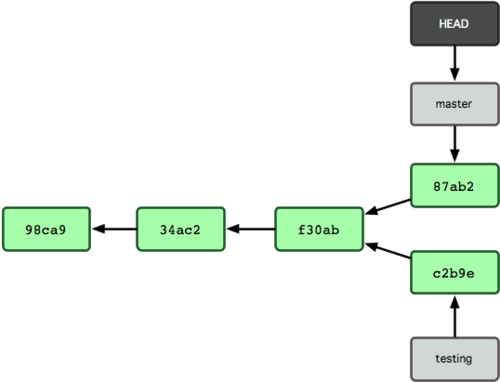
\includegraphics[width=6cm]{figs/rama_simple}
\end{center}
\end{figure}
\begin{tiny}
\begin{flushright}
Gráfico:git-scm.com
\end{flushright}
\end{tiny}

\end{minipage} \hfill
\

\begin{itemize}
\begin{small}
\item
Cada caja verde respresenta un estado de sistema de ficheros.
Git le llama \emph{objeto commit}, informalmente podemos
llamarle \emph{foto} (\emph{snapshot})
\item
Cada objeto commit apunta al objeto del que procede, su objeto
\emph{padre}. Por tanto, el tiempo avanza en sentido contrario a las flechas
\item
\end{small}
\end{itemize}
\end{frame}


%%---------------------------------------------------------------
\begin{frame}[fragile]
\frametitle{}
\begin{itemize}
\item
Cada objeto commit se identifica por un \emph{checksum} SHA1
\item
Si cada \emph{padre} tiene un solo \emph{hijo}, el desarrollo es lineal
y el sistema tiene una única rama (\emph{branch}): la rama \emph{master}
\item
En cierto momento del desarrollo, un padre puede tener un segundo hijo. Esto
crea una nueva rama, independiente de la anterior, con desarrollo paralelo. 
En el ejemplo anterior, la rama se llama \emph{testing}
\item
Para saber en qué rama estamos en cada momento, git emplea un puntero, llamado
\emph{HEAD}

No debemos confundir HEAD con \emph{master}
\begin{itemize}
\item
\emph{master}: primera rama, rama principal, rama por omisión
\item
HEAD: rama en la que estamos actualmente
\end{itemize}

\end{itemize}

\end{frame}

%%---------------------------------------------------------------

\begin{frame}[fragile]
\begin{minipage}{5cm}
\begin{figure}
\begin{center}
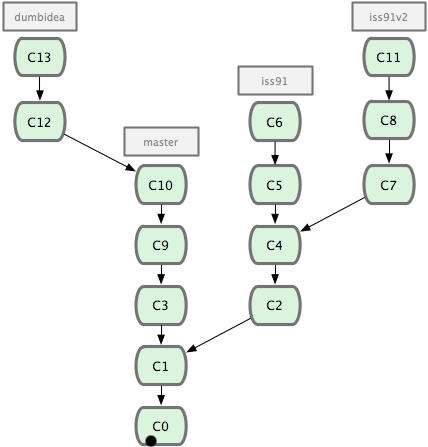
\includegraphics[width=6cm]{figs/rama_compleja}
\end{center}
\end{figure}
\begin{tiny}
\begin{flushright}
Gráfico:git-scm.com
\end{flushright}
\end{tiny}

\end{minipage} \hfill
\

\begin{itemize}
\begin{small}
\item
En otros sistemas de control de versiones, crear una rama
es bastante costoso
\item
Pero en git las ramas son muy eficientes y baratas, git anima
a crear muchas ramas, que luego pueden fusionarse automáticamente

\end{small}
\end{itemize}
\end{frame}



%%---------------------------------------------------------------
\begin{frame}[fragile]
\frametitle{}
\begin{itemize}
\item
\verb|git br| 
\footnote{Recuerda que br y co no son órdenes estándar de git,
sino alias que hemos creado para branch y checkout}

Muestra todas las ramas. Marca con un asterisco la actual
\item
\verb|git br nueva_rama|

Crea una rama nueva (pero no pasa a ella, HEAD se mantiene donde estaba)

\item
\verb|git co nueva_rama|

Pasa a la nueva rama (hace que HEAD apunte a la rama)


\end{itemize}

\end{frame}

%%---------------------------------------------------------------

%%---------------------------------------------------------------
\begin{frame}[fragile]
\frametitle{Recuperación de commits antiguos}

Al recuperar un estado antiguo, 
el sistema queda en una situación especial.
Obviamente, un estado pasado no se puede modificar sin más, porque los
hijos de ese estado resultarían inconsistentes

\begin{itemize}
\item
Una solución (que no usa git) podría ser dejar
los ficheros en modo \emph{read only}
\item
Lo que hace git es distinto: al retroceder a un estado pasado,
el sistema sale de la rama en la que se encontraba y pasa a un
estado especial, no asociado a ninguna rama


  \begin{tiny}
  \begin{verbatim}
koji@mazinger:/tmp/repo.01$ git co a3f9ba6c6f6e
Note: checking out 'a3f9ba6c6f6e'.

You are in 'detached HEAD' state. You can look around, make experimental
changes and commit them, and you can discard any commits you make in this
state without impacting any branches by performing another checkout.

If you want to create a new branch to retain commits you create, you may
do so (now or later) by using -b with the checkout command again. Example:

  git checkout -b new_branch_name

HEAD is now at a3f9ba6... Modifica esto y lo otro
  \end{verbatim}
  \end{tiny}

\end{itemize}
\end{frame}


%%---------------------------------------------------------------
\begin{frame}[fragile]
\frametitle{}
\begin{itemize}

\item
En un \emph{viaje al pasado} podemos consultar o modificar cualquier
cosa, pero los cambios no se almacenan en ningun sitio. A menos que
decidamos crear una nueva rama (y pasar a ella)

\verb|git br rama_nueva |

\verb|git co rama_nueva |
\footnote{Recuerda que br y co no son órdenes estándar de git,
sino alias que hemos creado para branch y checkout}
\item
Para \emph{volver al presente}, extraemos la rama que deseemos. Por ejemplo,
la rama master

\verb|git co master|


\end{itemize}
\end{frame}


%%---------------------------------------------------------------
\section{Repositorios Remotos}
%%---------------------------------------------------------------
\begin{frame}[fragile]
\frametitle{Repositorios remotos}
\begin{itemize}
\item
La principal característica de los VCS de 4ª generación
es que son distribuidos: un repositorio local se puede
sincronizar con un repositorio remoto
\item
Los repositorios se pueden organizar con muy diversas
topologías, pero la básica es una topología en estrella
con 1 maestro y n esclavos

\begin{itemize}
\item
Topologías más complejas suelen incluir varios niveles
jerárquicos de maestros
\item
Los esclavos no son simples réplicas del maestro, los cambios de
los esclavos se propagan al maestro

El maestro es maestro porque todos los cambios pasan a través
de él
\end{itemize}

\end{itemize}

\end{frame}

%%---------------------------------------------------------------

%%---------------------------------------------------------------
\begin{frame}[fragile]
\frametitle{}
Un repositorio \emph{maestro} es un repositorio un poco especial porque
es de tipo \emph{bare} (vacío)

\begin{itemize}
\item
Se trata de un repositorio contra el que 
no se pueden hacer ni recuperar commits
directamente, solo se usa para sincronizar otros repositorios

\item
No tiene ficheros ordinarios a la vista, 
solo contiene los 
ficheros que normalmente
están dentro del directorio .git
\item 
Por convenio, los repositorios maestros son directorios
con la extensión \verb|.git|

\end{itemize}

\end{frame}



%%---------------------------------------------------------------
\begin{frame}[fragile]
\frametitle{}
\begin{minipage}{1.5cm}
\begin{figure}
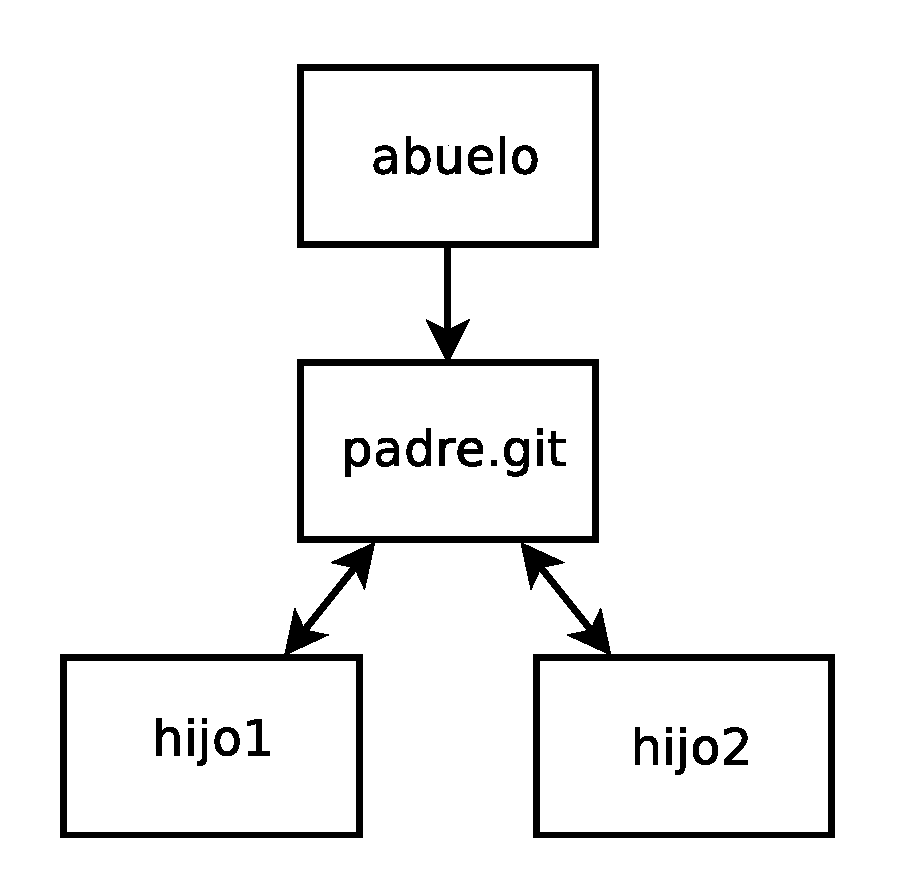
\includegraphics[width=4.0cm]{figs/familia_repos}
\end{figure}
\end{minipage} \hfill
\
\begin{minipage}{7.2cm}
\begin{itemize} 

\item
Al repositorio maestro le llamaremos \emph{padre.git} 

Es un repositorio especial, de tipo \emph{bare}
\item
A los repositorios esclavos les llamaremos \emph{hijos}
\item
El repositorio \emph{padre.git} se crea a partir de otro repositorio
al que llamaremos \emph{abuelo}

Una vez que el abuelo ha creado (por clonación) al padre, el
abuelo se puede borrar
\begin{itemize}
\item
O se puede cambiar la configuración del abuelo para que \emph{olvide}
lo que era 
y pase a ser un hijo más
\end{itemize}



\end{itemize}
\end{minipage}\hfill
\end{frame}

%%---------------------------------------------------------------

%%---------------------------------------------------------------
\begin{frame}[fragile]
\frametitle{}
Si queremos que un hijo se sincronice contra otro hijo
\begin{itemize}
\item
No podemos hacerlo 
directamente, siempre tiene que hacerse
a través de un 
\verb|padre.git|, de tipo \emph{bare}
\item
	Podemos hacer que este hijo tenga \emph{descendencia}
	y pase a ser un 
        \emph{abuelo2}, de forma que todo el proceso se repita

\end{itemize}

\end{frame}
%%---------------------------------------------------------------
\begin{frame}[fragile]
\frametitle{}
Creación de un repositorio \emph{abuelo} y un repositorio \emph{padre}

  \begin{scriptsize}
  \begin{verbatim}
#Creamos los directorios vacíos
mkdir abuelo
mkdir padre.git

# Entramos en el abuelo y hacemos de él un git
cd abuelo
git init

# En el abuelo creamos al menos un commit
# si no, el nieto tendrá problemas
touch primer_fichero  
git add primer_fichero
git ca -m "primer commit"

# Salimos del abuelo y creamos el padre
cd ..
git clone --bare abuelo padre.git
  \end{verbatim}
  \end{scriptsize}

\end{frame}


%%---------------------------------------------------------------
\begin{frame}[fragile]
\frametitle{}

\begin{enumerate}
\item
Creamos el repositorio hijo clonando el padre
\begin{itemize}
\item
El hijo puede tener acceso al padre o bien porque esté en el mismo
sistema de ficheros

  \begin{scriptsize}
  \begin{verbatim}
mkdir hijo
git clone padre.git hijo
  \end{verbatim}
  \end{scriptsize}

\item
O bien porque tiene acceso por ssh


  \begin{scriptsize}
  \begin{verbatim}
mkdir hijo
git clone usuario@maquina:/var/tmp/padre.git   hijo
  \end{verbatim}
  \end{scriptsize}
\item
O bien a través de HTTP, HTTPS o mediante 
un protocolo propio de git para acceso remoto
\end{itemize}

% rm -rf abuelo padre.git hijo
% mkdir abuelo padre.git hijo; cd abuelo; git init; cd .. ; git clone --bare abuelo padre.git;
% git clone padre.git hijo;

\item
Antes de usar el hijo por primera vez, es necesario indicar
qué rama del padre usará\footnote{Si en el padre no hay ningún commit,
este paso dará un error}
% error: src refspec master does not match any.


  \begin{scriptsize}
  \begin{verbatim}
cd hijo
git pull origin master
git push origin master
  \end{verbatim}
  \end{scriptsize}

\end{enumerate}

\end{frame}


%%---------------------------------------------------------------
\begin{frame}[fragile]
\frametitle{}
Una vez que el repositorio hijo está enlazado con el padre, podemos ejecutar (dentro del hijo)
\begin{itemize}
\item
\verb|git pull| 

Baja los cambios (\emph{tira})

\item
\verb|git push|

Sube los cambios (\emph{empuja})
\end{itemize}



\end{frame}
%%---------------------------------------------------------------
\begin{frame}[fragile]
\begin{minipage}{7cm}
\begin{figure}
\begin{center}
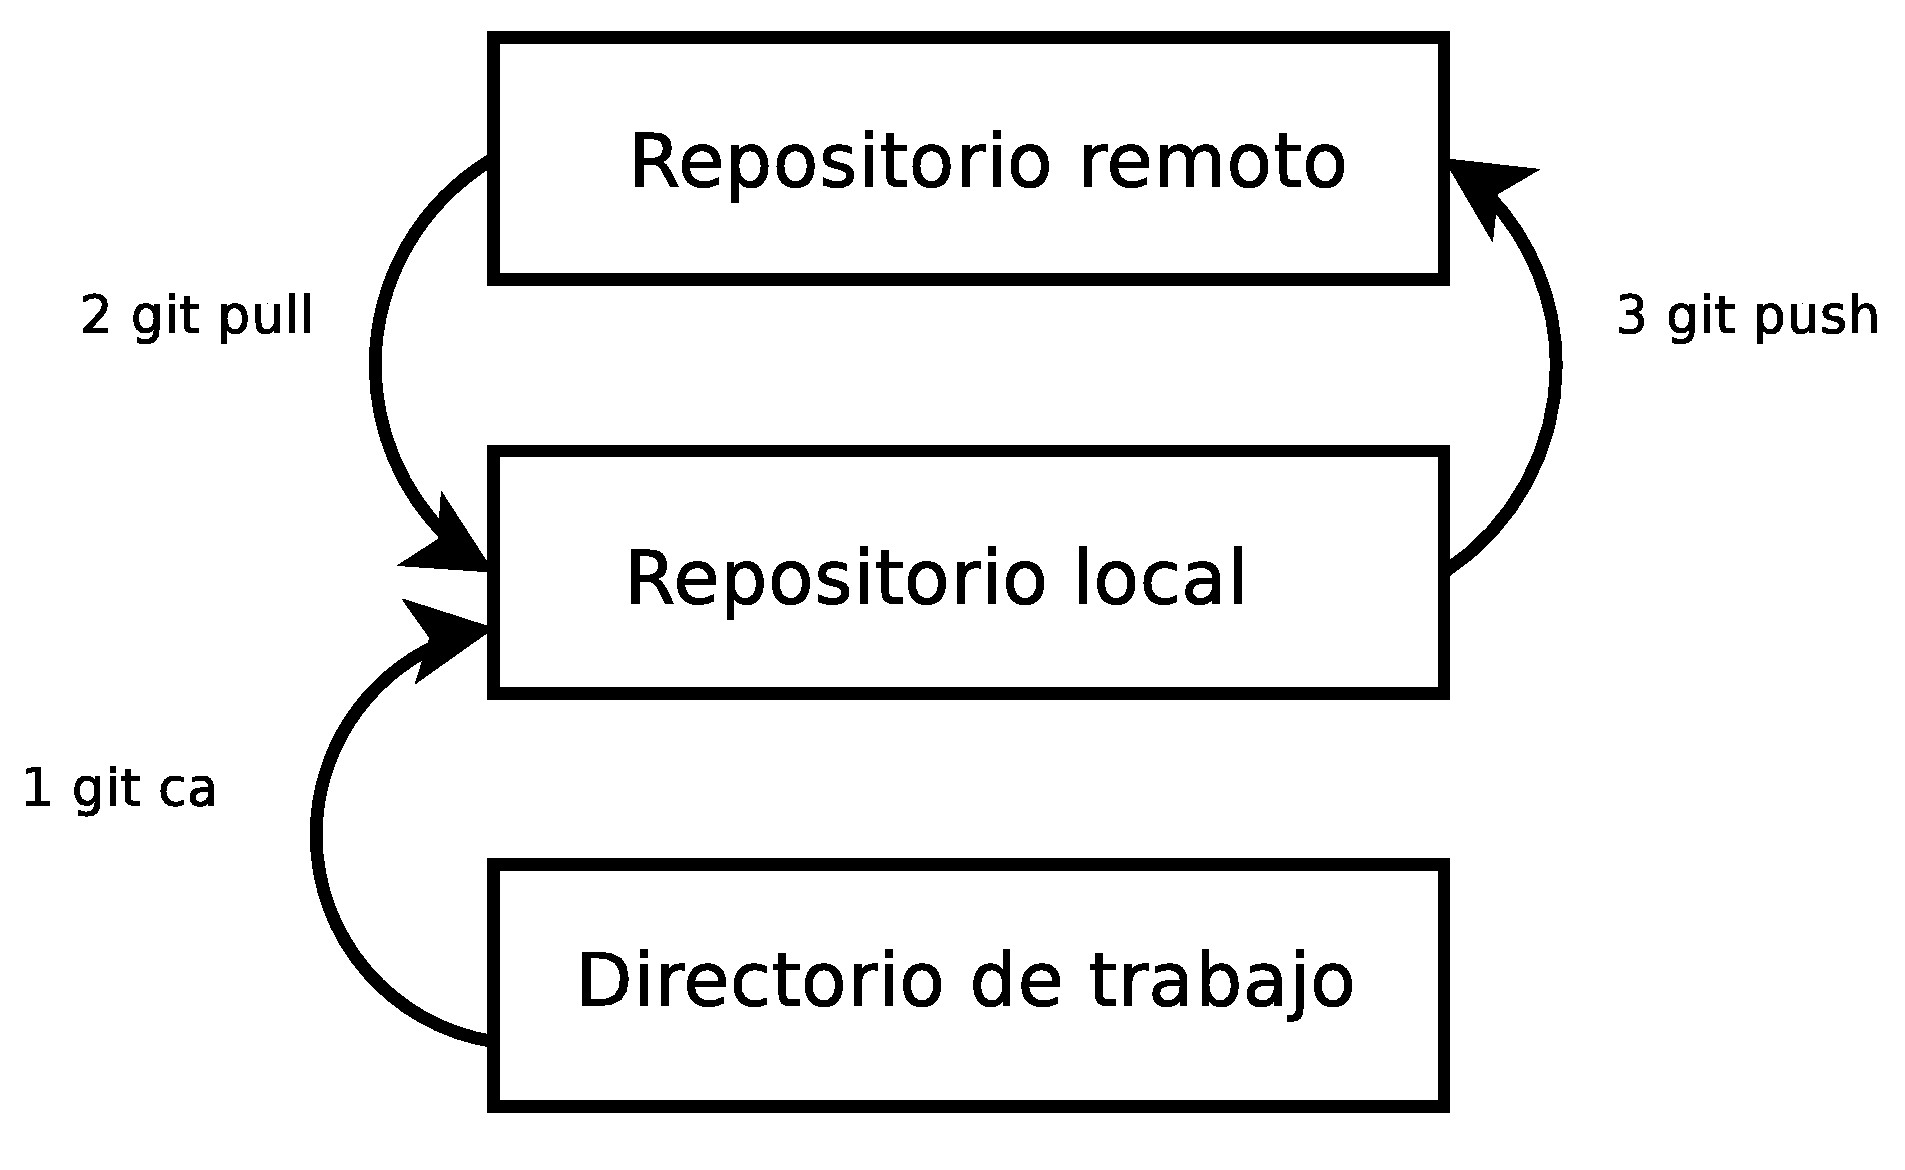
\includegraphics[width=6cm]{figs/ca_pull_push}
\end{center}
\end{figure}

\end{minipage} \hfill
\

Cada vez que queramos sincronizar el hijo con el padre,
es recomendable seguir estos tres pasos:
\footnote{No serán todos necesarios si en el repositorio remoto
no ha habido cambios o si hemos modificado ficheros no conflictivos, pero es
conveniente adquirir este hábito, al menos inicialmente}

  \begin{scriptsize}
  \begin{verbatim}
git ca    # Hago commit de todos los cambios
git pull  # Bajo (e integro) los cambios del padre
git push  # subo los cambios al padre
  \end{verbatim}
  \end{scriptsize}
\end{frame}


%%---------------------------------------------------------------
\begin{frame}[fragile]
\frametitle{}
Si olvidamos hacer \verb|ca| antes de \verb|pull|, es probable que 
obtengamos el siguiente error


  \begin{scriptsize}
  \begin{verbatim}
error: Your local changes to the following files would be overwritten by merge:
    fichero
Please, commit your changes or stash them before you can merge.
Aborting
  \end{verbatim}
  \end{scriptsize}
Git se niega a bajar el fichero, porque eso machacaría
un cambio local que no ha entrado en el repositorio

\end{frame}



%%---------------------------------------------------------------
\begin{frame}[fragile]
\frametitle{}
Si olvidamos el \verb|pull| antes de el \verb|push|, es similar
a decirle al repositorio padre 
\emph{aquí va mi repositorio, intégralo con el tuyo}

Esto no es válido, 
probablemente obtendremos el siguiente error

  \begin{scriptsize}
  \begin{verbatim}
 ! [rejected]        master -> master (non-fast-forward)
error: failed to push some refs to '/var/tmp/padre.git'
hint: Updates were rejected because the tip of your current branch is behind
hint: its remote counterpart. Merge the remote changes (e.g. 'git pull')
hint: before pushing again.
hint: See the 'Note about fast-forwards' in 'git push --help' for details
  \end{verbatim}
  \end{scriptsize}

Como hemos visto, lo correcto es hacer 

\verb|git ca; git pull; git push| 

que equivale a decir
\emph{meto mis ficheros en mi repositorio, dame tus cambios, yo los integro, cuando lo tenga ordenado,
lo subo}


\end{frame}


%%---------------------------------------------------------------
\begin{frame}[fragile]
\frametitle{}
Si queremos que el hijo se sincronice contra un padre en
una ubicación distinta, basta editar la línea
\verb|url| en el fichero de configuración local del repositorio
(\verb|.git/config| )

  \begin{scriptsize}
  \begin{verbatim}
[remote "origin"]
    fetch = +refs/heads/*:refs/remotes/origin/*
    url = ssh://milogin@192.168.1.12/var/tmp/padre.git
[branch "master"]
    remote = origin
    merge = refs/heads/master

  \end{verbatim}
  \end{scriptsize}
\begin{itemize}
\item
Si queremos que el abuelo pase a ser un hijo más, basta 
editar su fichero \verb|.git/config| para añadir
los dos párrafos anteriores
\end{itemize}

\end{frame}




%%---------------------------------------------------------------
\begin{frame}[fragile]
\frametitle{Conflictos}
Si dos hijos editan en paralelo el mismo fichero, se provocará
un conflicto que solo el usuario, a mano, podrá resolver


  \begin{scriptsize}
  \begin{verbatim}
auto-merging hola
CONFLICTO(contenido): conflicto de fusión en hola
Automatic merge failed; fix conflicts and then commit the result.
  \end{verbatim}
  \end{scriptsize}

Si se trata de ficheros de texto,
git combinará ambos.
Los bloques discrepantes
estarán enmarcados entre los símbolos \verb|<<<<<<<|,
\verb|=======| y \verb|>>>>>>>|

El usuario debe editar el fichero, añadirlo al repositorio
y sincronizarlos

  \begin{scriptsize}
  \begin{verbatim}
hola
<<<<<<< HEAD
Esta línea la escribo en hijo2
=======
Esta línea la escribo en hijo1
>>>>>>> 305e0f3a798338a9c990ffda032fe6322150102d

  \end{verbatim}
  \end{scriptsize}


\end{frame}

%%---------------------------------------------------------------
\begin{frame}[fragile]
\frametitle{Referencias}
\begin{itemize}
\item
Scott Chacon. Pro Git book. 

Disponible en \verb|http://git-scm.com/book|
\item
Git Immersion

\verb|http://gitimmersion.com|
\end{itemize}

\end{frame}
\end{document}
